\section{Dyna}\label{sec:Dyna_experiment}
Previously, we have demonstrated equivariant world models provide advantages over world models without an inductive bias.

However, for such techniques to be truly useful, the models must demonstrate an improvement in sample efficiency, while trained online in a full Dyna~\ref{algo:Dyna} setting.

In the same fashion as the Supervised-Dyna agents before, 128 agents were trained at each hyperparameter configuration initialized with independent random seeds. In comparison to the Supervised-Dyna experiments before agents are trained across 5 planning ratios and four values for the number of Dyna iterations. The planning ratio is much the same as before and controls the fraction of time spent planning to acting. The number of Dyna iterations controls the size of the buffer of transitions for both the transition model. As the number of timesteps is fixed, this provides a tradeoff between update frequency and dataset size for the transition model training.

\subsection{Results: CartPole Dyna}
\begin{figure}
	\centering
	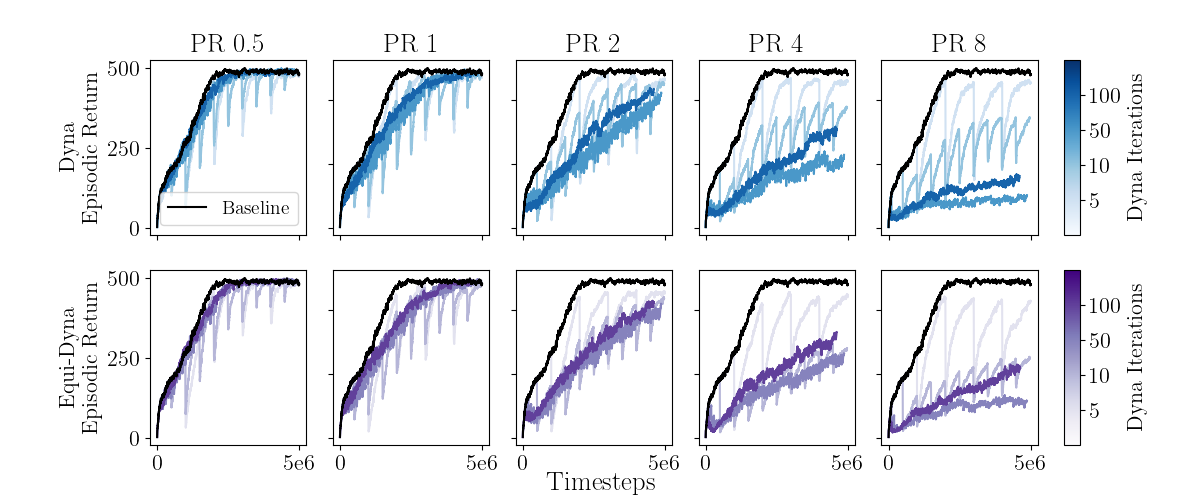
\includegraphics[width=\textwidth]{Figures/dyna_sweep_cp.png}
	\caption{A matrix of plots for mean episodic returns for the CartPole Dyna agents across 128 random seeds
		plotted against number of interaction time-steps in the MDP. The matrix varies planning ratio horizontally, and the top row is the conventional MLP transition model in blue. The equivariant transition models are all on the bottom row, in purple with }
	\label{fig:cp_dyna}
\end{figure}



